\section{Experiment}\label{foi.exp}
% ==================================================================================================
\subsection{Within- \vs Between-Partnership Heterogeneity}\label{foi.exp.xph}
For computing an average per-partnership probability of transmission ($B$),
\sref{foi.prior.bhet} clarified the interpretations of
\eqref{eq:B.wph} \vs \eqref{eq:B.bph} as modelling
within-partnership heterogeneity (WPH) \vs between-partnership heterogeneity (BPH), respectively.
As shown in \sref{app.math.misc.xph} (proof), $B_{\wph} \ge B_{\bph}$.
Here I explore under what conditions the ratio $B_{\wph}~/~B_{\bph}$ is maximized
--- \ie when does choosing the correct approach matter most.
For simplicity, I considered a single illustrative factor $f$
affecting $\alpha_f \in [0,1]$ proportion of sex acts ($1-\alpha_f$ are unaffected),
with relative probability of transmission $R_f \in [0.01,~10]$.
I~then computed $B_{\wph}$ and $B_{\bph}$ for $A \in [1,1000]$ total sex acts,
using a per-act probability of transmission $\beta = 0.34$\%
as a representative value for HIV \cite{Boily2009}.
\par
\begin{figure}
  \centering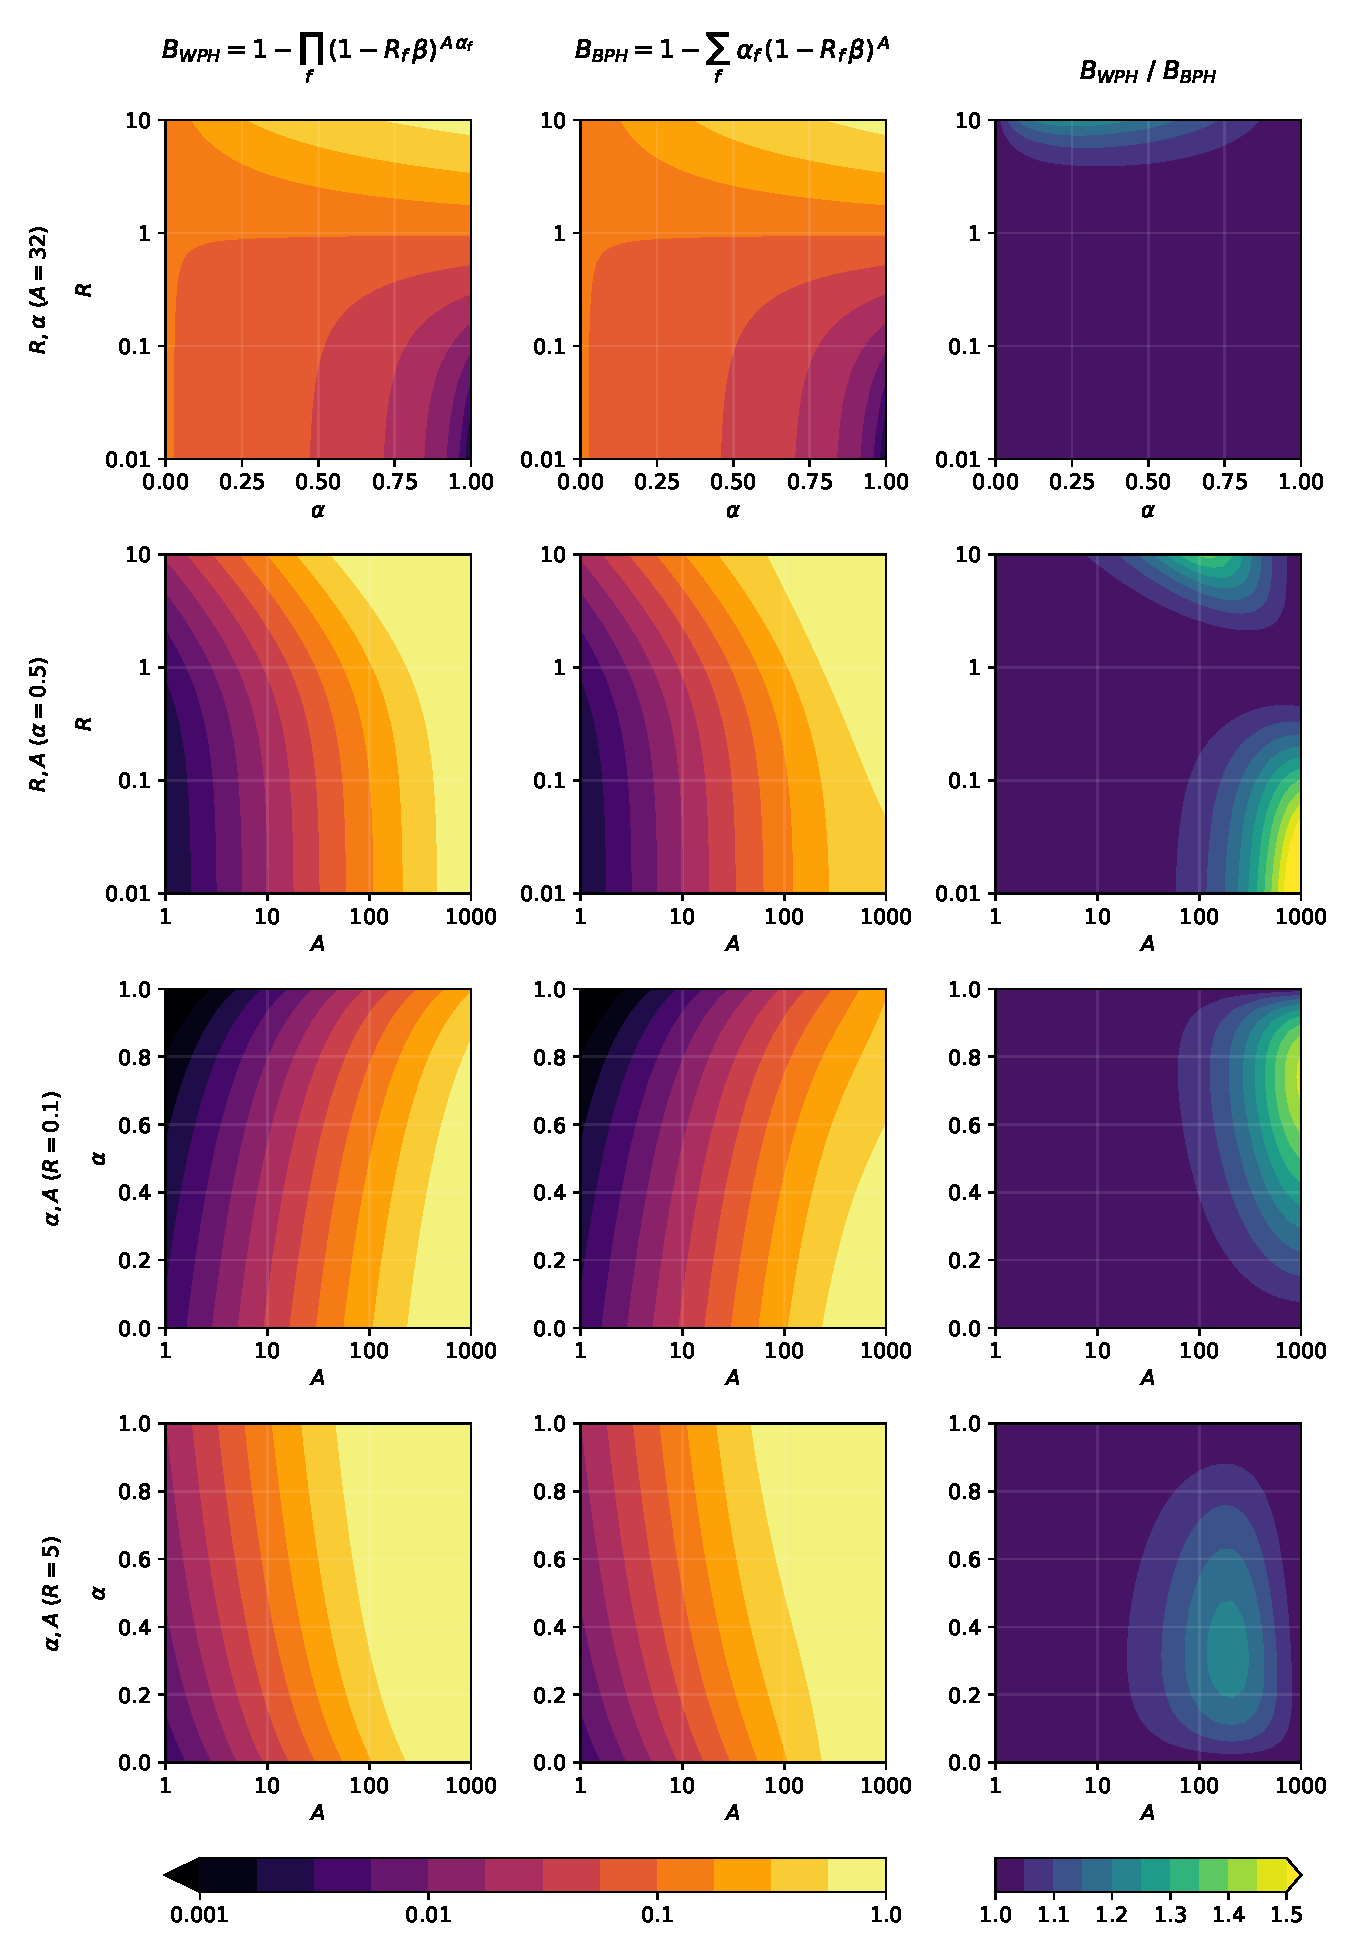
\includegraphics[scale=.6]{B.xph.surf.pdf}
  \caption{Average per-partnership probability of transmission $B$
    given heterogeneity in the per-act probability of transmission $\beta$
    within \vs between partnerships}
  \label{fig:B.xph.surf}
  \floatfoot{
    $B$: probability of transmission per partnership (log scale colourmap);
    $\beta = 0.34\%$: probability of transmission per sex act (fixed) \cite{Boily2009};
    $A$: total sex acts per partnership (log scale);
    $\alpha_f$: proportion of sex acts affected by factor $f$ (linear scale);
    $R_f$: relative $\beta$ given factor $f$ (log scale);
    WPH: within-partnership heterogeneity;
    BPH: between-partnership heterogeneity.}
\end{figure}
\begin{figure}
  \centering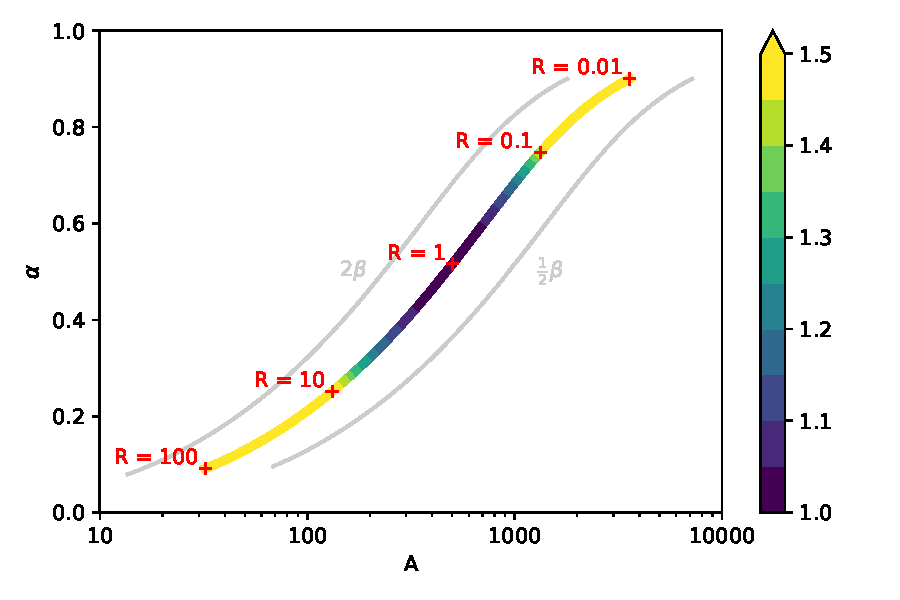
\includegraphics[scale=.6]{B.xph.max.pdf}
  \caption{Parameter values $(\alpha,A)$ which maximize the difference between
    the average per-partnership probability of transmission
    given within- \vs between-partnership heterogeneity}
  \label{fig:B.xph.max}
  \floatfoot{
    $B_{\wph}~/~B_{\bph}$: line colour;
    $\beta = 0.34\%$: probability of transmission per sex act (fixed) \cite{Boily2009};
    $A$: total sex acts per partnership (log scale);
    $\alpha_f$: proportion of sex acts affected by factor $f$ (linear scale);
    $R_f$: relative $\beta$ given factor $f$ (log scale);
    gray lines denote equivalent contours for $2\beta$ and $\frac12\beta$.}
\end{figure}
Figure~\ref{fig:B.xph.surf} illustrates four 2-dimensional cross sections of $B(R,\alpha,A)$
under WPH \vs BPH, and the ratio $B_{\wph} / B_{\bph}$;
the cross sections were at: $A = 32$, $\alpha = 0.5$, $R = 0.1$, and $R = 5$.
Based on these results, the difference between approaches can be summarized as:
\begin{itemize}
  \item negligible for $A < 10$, and small for $A < 100$
  \item increasing as $R$ gets farther from 1 ($R \rightarrow 0$ or $R \rightarrow \infty$)
  \item maximized by specific values of $(\alpha,A)$ for a given $R$, including
    $\alpha > \frac12$ for $R < 1$, and $\alpha < \frac12$ for $R > 1$
\end{itemize}
The specific values of $(\alpha,A)$ which maximize
the difference between approaches for a given $R$ and $\beta$
create a continuous curve (Figure~\ref{fig:B.xph.max}), which slowly tends towards
$\alpha \rightarrow 1, A \rightarrow \infty$ as $R \rightarrow 0$, and
$\alpha \rightarrow 0, A \rightarrow 0$ as $R \rightarrow \infty$.
The curve is sigmoidal for log-transformed $A$,
and shifts left with increasing $\beta$.
I did not derive an analytical expression, but it should be possible to do so.
In the context of HIV, the difference between approaches would be
larger for protective factors (\eg condoms)
affecting most of a large number of sex acts ($\alpha > 100$);
and likewise larger for risk-increasing factors (\eg anal sex)
affecting a minority of a moderate number of sex acts ($\alpha \approx 100$).
% ==================================================================================================
\subsection{Partnership Durations}\label{foi.exp.dur}
Figure~\ref{fig:dur.surf} TODO
\begin{figure}
  \centering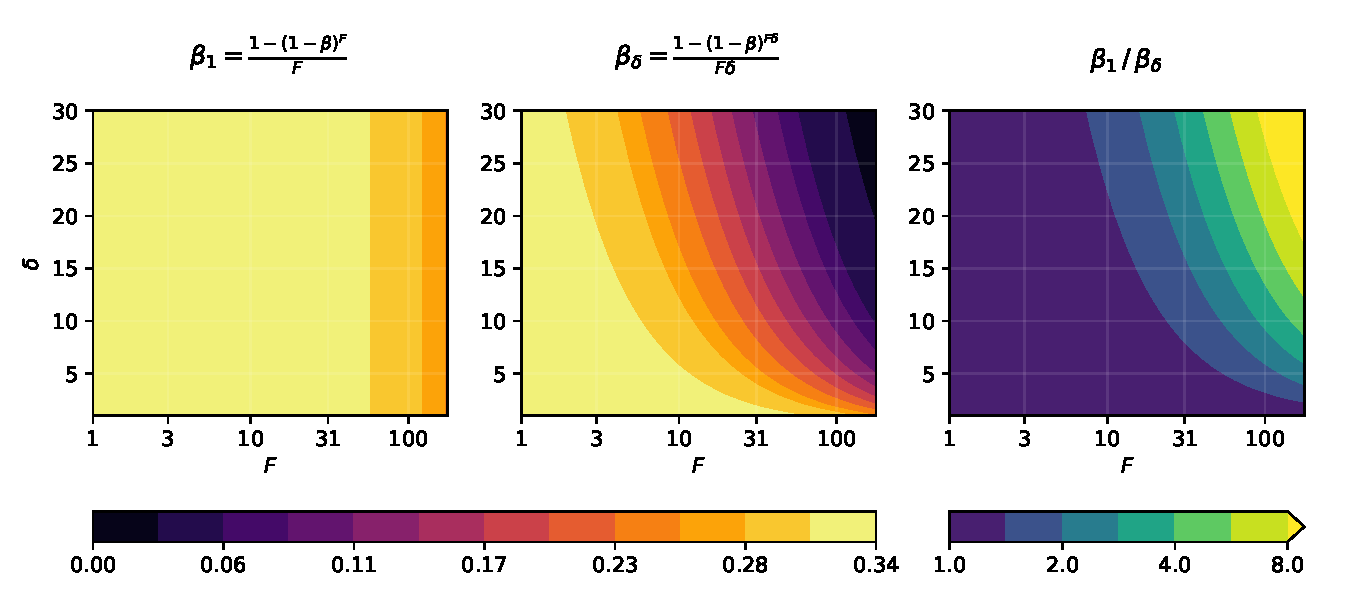
\includegraphics[scale=.6]{dur.surf.pdf}
  \caption{Effective probability of transmission per sex act
    over 1 year \vs total partnership duration}
  \label{fig:dur.surf}
  \floatfoot{
    $\beta = 0.34\%$: probability of transmission per sex act (fixed) \cite{Boily2009};
    $F$: frequency of sex per partnership (per year, log scale);
    $\delta$: partnership duration (years, linear scale);
    $\beta_1, \beta_\delta$: effective probability of transmission per sex act,
      for 1 year \vs total partnership duration, respectively.}
\end{figure}
% ==================================================================================================
\subsection{Full Model}\label{foi.exp.model}
